\documentclass[twocolumn,onesided,9pt]{article}

\usepackage{./Task32FlyerLatexStyle/Task32Flyer}
\usepackage{todonotes}

%% -----------------------------------
%% Document information
%% -----------------------------------
\def\pubdate{02 October 2019}
\title{IEA Wind Task 32: Wind Lidar}
\shorttitle{About Task 32}
\DOI{10.5281/zenodo.3482839}
\version{1.0}
\addbibresource{bibliography}

%% ===================================
%% Document starts
%% ===================================

\begin{document}

%% -----------------------------------
%% Title
%% -----------------------------------
\maketitle
\thispagestyle{cover}

%% -----------------------------------
%% Introductory text
%% -----------------------------------
{\Large\noindent%
We are a community dedicated to identifying and mitigating the barriers to the adoption of wind lidar for wind energy applications
}
\vskip 6pt

Wind lidar has many applications for wind energy that span all technology readiness levels. Task 32 connects researchers, product vendors, and end users, with the aim of supporting technology transfer.

% -----------------------------------
% Importance
% -----------------------------------
\section*{The importance of wind lidar for wind energy}
Wind lidar have many different applications for wind energy. In their simplest form they can supplement or replace met masts on land and offshore, but they can also be used to provide the data to control wind turbines or entire wind farms (Fig. \ref{fig:lotsOfLidar}), or to support research in other fields.

\begin{figure}[htb]
    \centering
    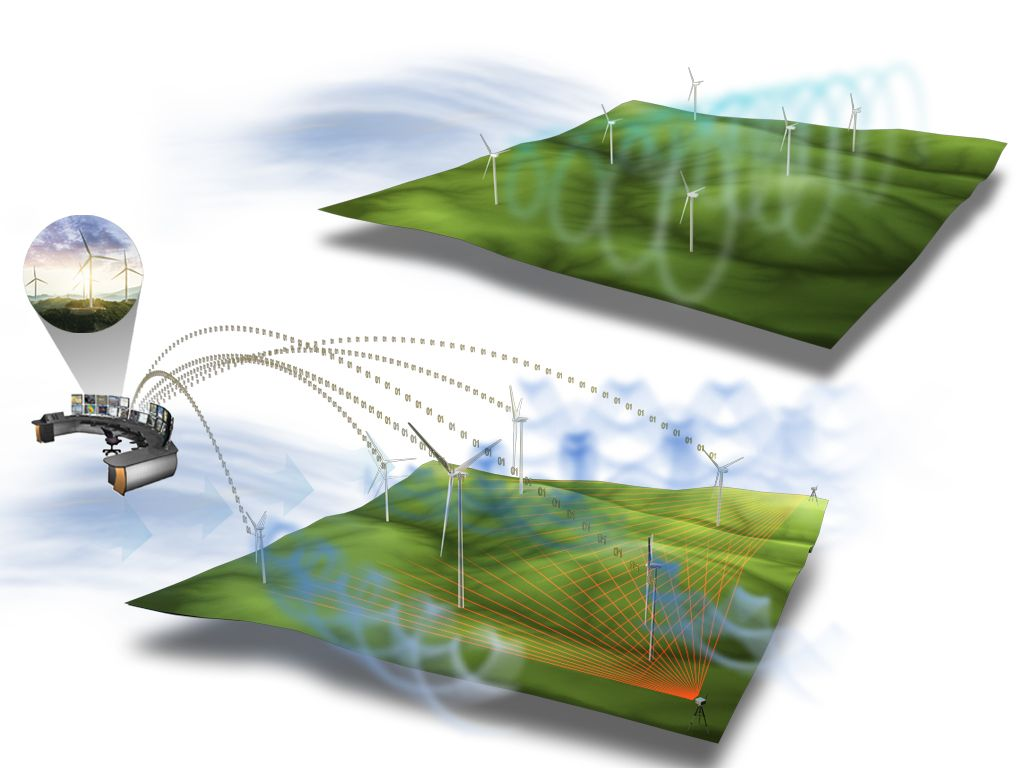
\includegraphics[width=\linewidth]{graphics/NRELTP-5000-68123-Fig4.jpg} 
    \caption{Wind lidar can be used to give unprecedented insight into the wind conditions in and around a wind plant and allow control. \citep[Figure from ][]{TP-5000-68123}}
    \label{fig:lotsOfLidar}
\end{figure}

Achieving this needs four things:
\begin{enumerate}
    \item \textbf{Standards} that give users more confidence in the devices, data, and their interpretation;
    \item \textbf{Experts} who understand wind lidars;
    \item \textbf{Data tools} to help the best from lidar data;
    \item \textbf{Better physics models} to help interpret lidar data.
\end{enumerate}

% -----------------------------------
% Why IEA Wind
% -----------------------------------
\section*{Why "IEA Wind ..."?}
Task 32 is one of several international collaborative research tasks that are enabled by the International Energy Agency (IEA) Technology Collaboration Programme (IEA Wind TCP). IEA Wind is a vehicle for member countries to exchange information on the planning and execution of large-scale wind system projects and to undertake co-operative research and development projects called Tasks or Annexes.

The decision to start a Task therefore recognises the potential for international co-operation to make a difference in a research field. It also means that the outcomes from a Task are subject to scrutiny by all of the members, ensuring quality and relevance.

% -----------------------------------
% Goals
% -----------------------------------
\section*{Our goals}
Our overarching goal is to identify and mitigate the barriers to adoption of wind lidar for wind energy. Because wind lidar are used in many different applications through the life cycle of a wind plant we have identified goals for each phase of the life cycle:
\begin{itemize}
    \item \textbf{Preconstruction \& turbine design}: Confident use of lidar in all terrains and offshore to provide all of the data needed to design and install wind turbines
    \item \textbf{Construction \& commissioning}: Community consensus on ways to use wind lidar to support power performance measurement and yaw alignment in all types of terrain and offshore
    \item \textbf{Operations}: Create common understanding of the benefits and limits of lidar measurements for wind turbine / plant control. Improve lidar systems and data processing using this understanding.
    \item \textbf{Data, tools, \& standards}: Develop and deploy community tools to create, support, and build on a common framework for executing all parts of a lidar project in all phases of a wind energy development.
\end{itemize}

% -----------------------------------
% Members
% -----------------------------------
\section*{Our members}
Task 32 is open to anyone from any IEA Wind member country that has agreed to the goals of the Task and agrees to support the Task. Task 32 is currently supported by financial contributions from 16 organisations in 12 countries (Austria, Canada, China, Denmark, France, Germany, Japan, Korea, the Netherlands, Norway, United Kingdom, and the USA).

Since the Task started in 2011, more than 400 people from 30 countries have taken part in our events. Of those, around 50\% identified themselves as being from industry, and the rest were in government roles or were academics.
\clearpage
% -----------------------------------
% How we work
% -----------------------------------
\section*{How we work}
Task 32 is led by an Operating Agent, currently \href{https://www.ifb.uni-stuttgart.de/forschung/windenergie/}{Stuttgart Wind Energy at the University of Stuttgart} and the \href{https://hs-flensburg.de/node/3513}{Wind Energy Technology Institute at the Flensburg University of Applied Sciences}. An Advisory Board works with the Operating Agents to help keep activities relevant to the wind energy community.

The Task members use our annual meetings to identify and prioritise topics for the Task to investigate in the next one to two years. This allows us to respond to new trends and developments and leverage existing and near-term funding. We then hold topic-specific Workshops to identify issues that are important and identify possible solutions. Ad-hoc Working Groups then continue to work on these issues, and members are free to pursue other funding to carry out their own research and development. 

More information about our activities can be found on the \href{https://community.ieawind.org/task32/home}{Task 32 web site} and in the Task 32 Roadmap \cite{Clifton_2019_3374354}.

% -----------------------------------
% Achievements
% -----------------------------------
\section*{What we've achieved}
Task 32 has contributed significantly to the adoption of wind lidar for wind energy applications \cite{Clifton_2018_a}. We have:
\begin{itemize}
    \item Developed frameworks for the deployment and use of wind lidar for land-based wind resource measurements \cite{Clifton_2013_RP15} and for many common use cases for floating lidar systems \cite{Bischoff_2017_a}.
    \item Created solutions to enable the certification of wind turbines with lidar -assisted control \cite{Schlipf_2018}.
    \item Explored ways in which lidar could be used for energy forecasting \cite{Wuerth2019_Energies}.
    \item Suggested new approaches to building and operating wind lidar and integrating them into digital wind energy processes \cite{clifton_2019_3414197, clifton_2019_3447756}.
\end{itemize}

% -----------------------------------
% Working Towards
% -----------------------------------
\section*{Where we're going}
We have identified several important topics for 2020 and beyond:
\begin{itemize}
    \item Mitigating the effect of complex terrain on power performance measurements by using nacelle-mounted lidar
    \item Investigating the use of measurements in the induction zone for power performance measurements
    \item Understanding the uses for wind lidar in cold climates
\end{itemize}

% -----------------------------------
% Get involved
% -----------------------------------
\section*{How to get involved}
Come to an event! We welcome participants at our events from any of Task 32's member countries, and encourage observers from the rest of the IEA wind member countries. We'd love to hear your opinions about what we should be doing, or ideas for solutions that benefit the whole community. We ask only that you bring enthusiasm, openness, and a focus on solutions.

%% -----------------------------------
%% References
%% -----------------------------------
%\section*{References}
% bibliography
\newpage
\label{sec:References}
\addcontentsline{toc}{section}{References}
\defbibnote{openaccess}{The following documents are all open access.}
{\small
\printbibliography[prenote=openaccess]
}

%% -----------------------------------
%% Outlined block of smaller text
%% -----------------------------------
\begin{tcolorbox}[width=1.0\columnwidth,
                  boxsep=0pt,
                  left=3pt,
                  right=3pt,
                  top=3pt,
                  arc=0pt,
                  boxrule=0.5pt,
                  toprule=0.5pt,
                  colback=white,
                  coltext=TextGrey
                  ]
{\footnotesize
This white paper was self published by IEA Wind Task 32.

%% -----------------------------------
%% IEA WIND AND TASK 32
%% -----------------------------------
\begin{tabular}{m{0.3\columnwidth}m{0.6\columnwidth}}
    % IEA Wind * DO NOT EDIT THIS TEXT *
    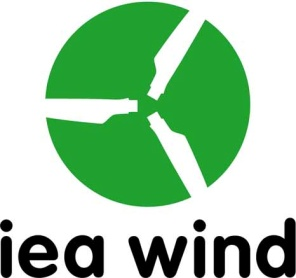
\includegraphics[height=2cm]{graphics/IEAWind_logo.jpg} &
    The International Energy Agency is an autonomous organisation which works to ensure reliable, affordable and clean energy for its 30 member countries and beyond. The IEA Wind Technology Collaboration Programme supports the work of 38 independent, international groups of experts that enable governments and industries from around the world to lead programmes and projects on a wide range of energy technologies and related issues.  %
    \\
    % Task 32 * DO NOT EDIT THIS TEXT *
    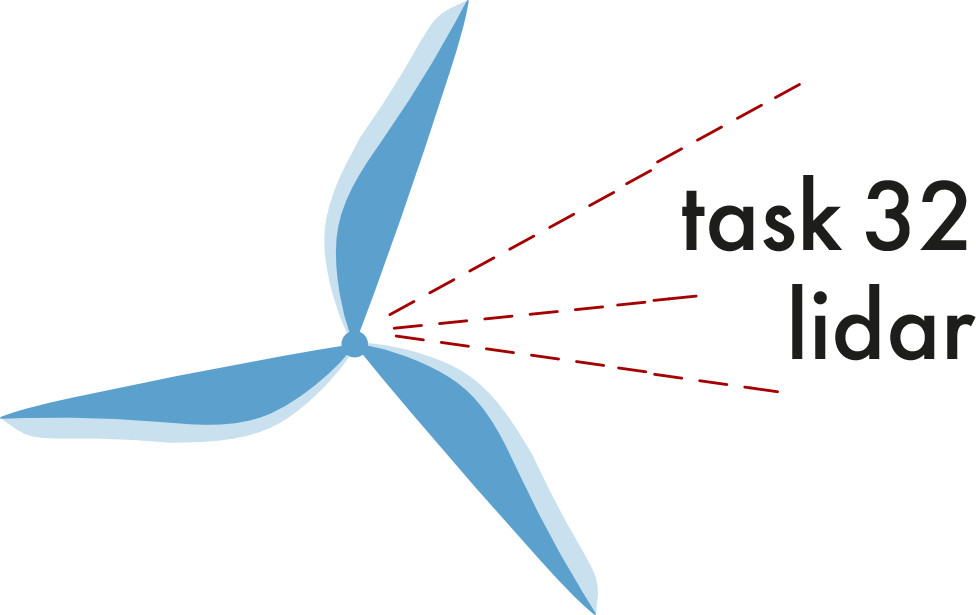
\includegraphics[height=1.5cm]{graphics/Task32_logo.jpg} &
    \href{https://community.ieawind.org/task32/home}{IEA Wind Task 32} exists to identify and mitigate the barriers to the deployment of wind lidar for wind energy applications.
\end{tabular}%

%% -----------------------------------
%% For more information
%% -----------------------------------
% N.B. do not add line breaks between the next items
\textbf{For more information:} See the  \href{https://community.ieawind.org/task32/home}{Task 32 website}.
%% -----------------------------------
%% Authors
%% -----------------------------------
\textbf{Author team:} %
Andrew Clifton (Task 32 Operating Agent, University of Stuttgart, Germany), %
David Schlipf (Task 32 operating Agent, Flensburg University of Applied Sciences, Germany).
%% -----------------------------------
%% Reviewers
%% -----------------------------------
%\textbf{Reviewers:} %
% first last (short affiliation), %
% first last (short affiliation).
%% -----------------------------------
%% Images
%% -----------------------------------
\textbf{Images:}
Banner, left to right: \href{https://unsplash.com/@alexkixa}{Alexandre Debiève on Unsplash}, \href{http://ifb.uni-stuttgart.de}{SWE U. Stuttgart}, \href{https://unsplash.com/@markusspiske}{Markus Spiske on Unsplash}.
}

%% -----------------------------------
%% End of highlighted block
%% -----------------------------------
\end{tcolorbox}

\end{document}
